\documentclass[12pt,fleqn]{article}
\setlength{\parindent}{0pt}
\usepackage{graphicx}
\usepackage{listings}
\usepackage[latin5]{inputenc}
\setlength{\parskip}{8pt}
\setlength{\parsep}{0pt}
\setlength{\headsep}{0pt}
\setlength{\topskip}{0pt}
\setlength{\topmargin}{0pt}
\setlength{\topsep}{0pt}
\setlength{\partopsep}{0pt}
\setlength{\mathindent}{0cm}

\begin{document}
S�n�rl� Elementler Metodu (Finite Elements Method)

Bu metot differansiyel, kismi differansiyel denklemleri (partial differential
equations) yaklasiksal olarak modelleme ve cozmenin yontemleridir.

Formul: Baslangic denklemi

\[ \frac{-d}{dx} \bigg( c(x) \ \frac{du}{dx} \bigg) = f(x) \]

Iki tarafi da  $v(x)$ ile carpiyoruz ve 0 to 1 sinirlariyla entegralini aliyoruz.

\[ \int_0^1 \frac{-d}{dx} \bigg( c(x) \ \frac{du}{dx} \bigg) v(x)dx = \int_0^1 f(x)v(x)dx \]

Parcali entegral (integration by parts) formulu soyledir:

\[ \int y \ dz = y  z \int z \ dy \]

Ana formulun bolumlerini, parcali entegrale gore bolusturursek:

\[ dz = \frac{-d}{dx} \bigg( c(x) \ \frac{du}{dx} \bigg) dx  \]

\[ z = - c(x) \ \frac{du}{dx}  \]

\[ y = v(x)  \]

\[ dy = \frac{dv}{dx}dx \]

Yukarida $dz$ icinde $dx$ ve $\frac{1}{dx}$ birbirini iptal eder. Parcali
entegral formulunun sag tarafina gore yerlerine koyarsak:

\[ \int_0^1 v(x)dx \frac{-d}{dx} \bigg( c(x) \ \frac{du}{dx} \bigg) = - [v(x) c(x) \frac{du}{dx} \bigg]_{x=0}^{x=1} \int_0^1 c(x) \ \frac{du}{dx} \frac{dv}{dx}dx \]

Ustteki parcali entegral aciliminda sol taraf entegrale sinir
degerleri aldiginda, sag taraftaki $yz$ sonucunun ayni sinir
degerlerine tabi olduguna dikkat edelim.

Differansiyel denklemde sinir kosullari $x=1$ durumunda $c(1)u'(1)=0$,
ve $x=0$ durumunda $v(0)=0$ olarak biliniyor. O zaman ustteki
denklemin sol tarafinda $x=0$ ve $x=1$ kosullari icin tanimli bolum $0
- 0 = 0$ olacaktir ve denklemden atilabilir. Geriye kalanlar

\[ \int_0^1 c(x) \frac{du}{dx} \frac{dv}{dx} dx  = \int_0^1 f(x)v(x)dx \]

Bu fonksiyonu Galerkin adli bir matematikci bulmus, ``zayif form (weak
form)'' olarak adlandiriliyor.

Simdi diyelim ki n tane test fonksiyonu sectik $\phi_1(x),..,\phi(n)$
ve bu fonksiyonlarin $U_j$ sayilari ile carpiminin toplamini, yani bir
tur kombinasyonunu $u(x)$ yerine kullanmaya karar verdik.

\[ U(x) = U_1 \phi_1+ ... + U_n\phi_n \]

O zaman

\[ U'(x) = U_1 \phi_1'+ ... + U_n\phi_n' \]

\[ = \sum_1^n U_j \frac{d\phi_j}{dx} \]

Simdi $du / dx$ yerine $U'(x)$ koyarsak

\[ \int_0^1 c(x) \bigg( \sum_1^n U_j \frac{d\phi_j}{dx}\bigg)  \frac{dV_i}{dx} dx  = \int_0^1 f(x)V_i(x)dx \]

Dikkat edelim, $v(x)$ yerine $V_i(x)$ kullandik. Ustteki formul her i icin yeni
bir formul ``uretecek''. Niye $V_i$? Zayif formdaki $v(x)$ formulunu de zaten
biz uydurmustuk, yani $v(x)$ biz ne istersek o olur. O zaman bu fonksiyonu n
tane formul uretmek icin bir numara olarak kullaniliyoruz, n tane formul olunca
matrisin n x n elemanini doldurabilecegiz ve cozume erisebilecegiz. Ek not,
cogunlukla $V_i(x)$ icin $\phi_i$ formulleri kullaniliyor. 

Ayrica formuldeki $U_j$ kismini cekip cikartirsak ve bir vektor icine koyarsak,
geri kalanlar bir $K_{ij}$ matrisi icinde tutulabilir. 

\[ K_{ij} = \int_0^1 c(x) \frac{d\phi_j}{dx} \frac{dV_i}{dx} dx  \]

Sag taraf ayni sekilde i tane formul uretir

\[ F_i = \int_0^1 f(x)V_i(x)dx \]

Final formul matrix formunda basit bir sekilde temsil edilebilecektir. 

\[ KU = F \]

Ornek

Ornek olarak $-u'' = 1$ denklemini cozelim. Not: Differansiyel
denklemlerde sonuc bulmak demek bir ``fonksiyon'' bulmak
demektir. Normal cebirsel denklemlerde sonuc bulmak degiskenlerin
``sayisal'' degerini bulmak demektir. Birazdan bulacagimiz sonuc
$u(x)$ ``fonksiyonu'' olacak.

Eger denklem $-u''=1$ ise o zaman bu formulu ana forma uygun hale
getirmek icin $c(x) = 1$ olarak almamiz gerekir. $-u''=1$ denkleminde
esitligin sag tarafi 1 olduguna gore $f(x) = 1$ demektir.

Artik $\phi$ fonksiyonlarini secme zamani geldi. Bu fonksiyonlarin
``toplami'' hedefledigimiz fonksiyonu yaklasiksal (approximate) olarak
temsil edecek. Ornek olarak secebilecegimiz bir fonksiyon ``sapka
fonksiyonu (hat function)'' olarak bilinen ucgen fonksiyonlar
olabilir. Alttaki figurde bu fonksiyonlari goruyoruz.

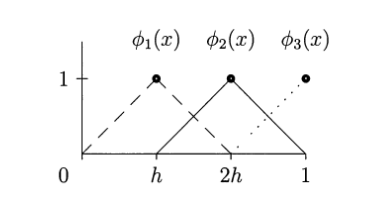
\includegraphics[height=3cm]{fem_hat.png}

Bu figurde x ekseninin h buyuklugundeki parcalara bolundugunu goruyoruz. 

Entegralleri hesaplayalim

\[ F_1 = \int_0^1 V_1(x)dx \]

Daha once $V_1$ ve $\phi_1$'i ayni kabul ettigimizi belirtmistik. 

Yukaridaki entegralin aslinda bir alan hesabi yaptigini
goruyoruz. Sinirlar $0$ ve $1$ arasinda, ama $2h$ otesinde zaten
$\phi_1$ fonksiyonu yok. $\phi_1$'in alani nedir? Alan ucgenin alani:
Taban carpi yukseklik bolu 2: $2h$, yuksekligi $1$, o zaman alan $(2h
\times 1) / 2 = 1/3$

Benzer mantikla bakarsak, $F_2$ ile $F_1$ ayni, yani $1/3$. $F_3$ ise
onlarin yarisi, yani $1/6$.

$K_{ij}$ nasil hesaplanacak? $c(x) = 1$ oldugu icin formulden
cikarilabilir ve $V_1$ ve $\phi_1$'in ayni olduguna soyledik:

\[ K_{ij} = \int_0^1 c(x) \frac{d\phi_j}{dx} \frac{dV_i}{dx} dx \]

\[ K_{11} = \int_0^1 \bigg( \frac{dV_1}{dx} \bigg) ^2 dx  \]

$dV_1/dx$ nedir? Birinci sapka fonksiyonunun turevidir. Bu tureve
bakarsak, $0$ ve $h$ arasinda arti egim (slope) $1/h$, $h$ ve $2h$
arasinda eksi egim $-1/h$ oluyor. Ama kare aldigimiz icin sonuc ayni,
$1/h^2$. O zaman h = 1/3 olduguna gore $1/(1/3)^2$, yani $dV_1/dx =
9$.

\[ K_{11} = \int_0^{2/3} 9 dx = 9x \ \bigg|_0^{2/3} = (9)(2/3) - 0 = 6 \]

$K_{22}$ seklen ayni fonksiyon parcasini temel aldigi icin ayni degere
sahip: 6. $K_{33}$ onlarin yarisi, esittir 3.

$K_{12}$ farkli egimlerin carpimi anlamina gelir, yani $V_1'$ ile
$V_2'$ carpimi olur. Bu iki fonksiyona bakalim, 0 ile h arasinda $V_2$
yok, egim 0. Ikisinin de sifir olmadigi, carpimda kullanilabilecek bir
egiminin oldugu tek aralik h ve 2h arasi. Burada $V_1' = -3, V_2 = 3$.

\[ K_{12} = \int_{1/3}^{2/3} (3)(-3) dx = -9x \bigg|_{1/3}^{2/3} = -6 - (-3) = -3 \]

Ayni sekilde $K_{23} = -3$. Ama $K_{13} = 0$ cunku hic cakisma yok.

Matrisi doldurursak, 

\[ 
KU = F \\ \\
\left[ \begin{array}{ccc}
    6 & -3 & 0 \\
    -3 & 6 & -3 \\
    0 & -3 & 3     
\end{array} \right]
\left[ \begin{array}{c}
    U_1 \\
    U_2 \\
    U_3
\end{array} \right] =
\left[ \begin{array}{c}
    1/3 \\
    1/3 \\
    1/6
\end{array} \right]
 \]

Python kodu 

\begin{lstlisting}[language=Python]
import numpy as np

K = [[6., -3., 0],
     [-3., 6., -3.],
     [0., -3., 3.]
     ]

f = [1./3., 1./3., 1./6.]

print np.linalg.solve(K,f)
\end{lstlisting}

Rapor edilen degerler $0.277, 0.44, 0.5$'in bu denklemin bilinen cozumu $u(x) =
x - \frac{1}{2}x^2$ ile 0, h, 2h noktalarinda (mesh points) birebir uyum
gosterdigini goruyoruz. Yani yaklasiksal olarak differansiyel denklemi cozmeyi
basardik.

{\em Kaynaklar}

Strang, G., Computational Science and Engineering, 2007

\end{document}





